%
\section{Conditional Branch Characterization}
%
Since the proper handling of conditional branches is important
in any microarchitecture that spawns additional speculative
paths for unresolved branches, some attention is given
towards characterizing their behavior.  
We focused
on five benchmark programs for characterizing branch behavior.
The benchmark programs explored along with some statistics 
are given in Table \ref{tab:benches}.

\begin{table}
\begin{center}
\caption{Benchmarks Analyzed and Some Statistics.}\label{tab:benches}
\begin{tabular}{|c|c|c|c|c|}
\hline 
benchmark&
prediction accuracy&
avg. L1 miss rate&
dynamic cond. brach-es & forward branches\\
\hline
\hline 
go&
72.1\%&
96.6\%&
9.0\% & 89\%\\
\hline 
gap&
94.5\%&
98.9\%&
6.2\% & 91\%\\
\hline 
bzip&
90.5\%&
98.5\%&
7.0\%&81\%\\
\hline 
gzip&
85.4\%&
97.0\%&
8.8\%&85\%\\
\hline 
parser&
92.6\%&
98.3\%&
13.0\%&85\%\\
\hline
\end{tabular}
\end{center}
\end{table}

The {\tt go} benchmark is from the SpecInt-95 suite while the rest
are from the SpecInt-2000 suite.
All benchmark programs were executed for 100 million instructions
as a warm up for the simulator.  After this they were simulated
for 500 million instructions for which all data was collected.
The predictor used was a PAg with
a PBHT of 1024 entries and a GPHT size of 4096 entries.
The L1 cache was a 32kB, 2-way set associative, with 1 cycle hit
penalty and a 20 cycle miss penalty.

We were interested
in the size of the branch domains for both all branches
dynamically executed in the programs as well as for those branches 
that contribute most to mispredictions.  The branch domain size
is the number of instructions on the not-taken output path
before a join with the target instruction of the branch.
Figure \ref{fig:numbranches} shows a percent distribution of
the number of dynamic branches versus 
branch domain size.  
Figure \ref{fig:mispredictions} shows a percent distribution of
the number of branch mispredictions versus
branch domain size.
From these two figures it can be seen 
that a large fraction of total mispredictions 
is due to branches with small domain
sizes. 
This is likely a valuable characteristic to exploit for
possible alternative speculative paths in our proposed
microarchitecture.  This is so since all of the branch domain
instructions for most
branches will be issued into the execution window allowing
for both branch outcomes to be executed simultaneously
in our microarchitecture.
To get a better understanding of how to handle different branches,
we proceeded to define four orthogonal characteristics
for conditional branches that might give us insight into
how they might be handled in the microarchitecture.
The four characteristics used to classify each conditional branch are :

\begin{figure}
\vspace{0.2 in}
\setlength{\epsfxsize}{10cm}%7
\centerline{\epsfbox{numbranches.eps}}
%\centering
%\epsfig{file=numbranches.eps,width=5.8in}
\caption{{\em Percent Distribution of Dynamic Branches versus
Branch Domain Size.} 
Shown are the percent dynamic branches that have a domain size
in instructions at or below a given value.}
\label{fig:numbranches}
\end{figure}

\begin{figure}
\vspace{0.2 in}
\setlength{\epsfxsize}{10cm}%7
\centerline{\epsfbox{mispredictions.eps}}
%\centering
%\epsfig{file=mispredictions.eps,width=5.8in}
\caption{{\em Percent Distribution of Branch Mispredictions
versus Branch Domain Size.} 
Shown are the percent branch mispredictions that have a domain
size in instructions
at or below a give value.}
\label{fig:mispredictions}
\end{figure}

\begin{itemize}
\item{execution frequency}
\item{branch predictability}
\item{direction of the branch target -- forward or backward}
\item{distance to the target of the branch}
\end{itemize}   

We classify each conditional branch as 
being either a high dynamic frequency branch
or a low dynamic frequency branch.  
If the conditional branch
is within the top 90\% of all dynamically executed conditional branches,
it is classified as a \textit{high} frequency branch, else it 
is \textit{low} frequency.
For each conditional branch, we also accumulate statistics on
its predictability.  Figure \ref{fig:bpdist} shows 
the percent distribution of branches versus prediction accuracy.
As can be seen, for most benchmarks
the branch predictability is distributed over a large range of values.
One implication of this is that we need the misprediction
penalties associated with most of the branches 
regardless of their predictability.

Another parameter that is also recorded is the direction of the branch 
which can simply
be either a 
\textit{forward} branch or a 
\textit{backward} branch.
Finally, the distance of the branch to 
the instruction at the
branch targer is computed and recorded.  The distance is measured
in instructions.  If the target of the branch is less than 170 instructions
from the branch itself, the branch is considered to have a 
\textit{near} target, else it is considered to have a
\textit{far} target.  The value of 170 instructions was chosen
because for many of the machine configurations that we will be
investigating, this number is approximately between one half of
the possible number of speculatively executed instructions
that can be in-flight and two thirds of the total possible number.
This will be clarified later.

\begin{figure}
\vspace{0.2 in}
\setlength{\epsfxsize}{10cm}%7
\centerline{\epsfbox{bpdist.eps}}
%\centering
%\epsfig{file=bpdist.eps,width=5.8in}
\caption{{\em Probability Distribution of Branches versus Prediction Rate.} 
Shown are the percentage of dynamic
branches with a predictability at or less than a given prediction
accuracy.}
\label{fig:bpdist}
\end{figure}
%
